\documentclass[10pt]{beamer}
% Beamer uses a standard paper size of 128x96mm

% ===== Packages =====
\usepackage[utf8]{inputenc}
\usepackage[T1]{fontenc}

\usepackage{graphicx}
\usepackage{tikz}  % TODO: utilisé pourquoi? (il est particulierement lent a compiler avec)
\usepackage{enumitem} % Custom lists
\usepackage{mathtools} % endlesssssss maths

\usepackage[backend=biber, autolang=other, style=phys, sorting=none]{biblatex}  % Citing
\addbibresource{../bibliography/bibliography.bib}
\makeatletter
\renewcommand\@makefnmark{\hbox{{\usebeamercolor[fg]{footnote mark}\usebeamerfont*{footnote mark}[\@thefnmark]}}}     %% to replace "[#1]" with "(#1)"
\makeatother
% ===== Typeface =====
\usepackage{mlmodern} % thicker math, do not touch

% \usepackage[sfdefault]{FiraSans} % peculiar but nice
% \usepackage{tgheros} % nice
\usepackage[sfdefault]{plex-sans} % nice
% \usepackage[sfdefault]{noto}
% \usepackage[sfdefault, light]{FiraSans} 
% \usepackage{helvet}
% \usepackage[sfdefault]{AlegreyaSans} % peculiar
% \usepackage{montserrat}
% \usepackage{raleway}
% \usepackage{avant} % nah
% \usepackage{tgadventor} % nah
% \usepackage{cmbright} % meh
% \usepackage{DejaVuSans} % big
% https://tug.org/FontCatalogue/sansseriffonts.html

% ===== Beamer theme =====
\usetheme{Boadilla} % other interesting built-in: Boadilla, CambridgeUS (if we want sections in header), Pittsburgh (super-plain)

\setbeamertemplate{footline}{   % only page number in footline
\hfill%
\usebeamercolor[fg]{page number in head/foot}%
% \usebeamerfont{page number in head/foot}%
\footnotesize%
    \setbeamertemplate{page number in head/foot}[framenumber]%
    \usebeamertemplate*{page number in head/foot}\kern1em\vskip4pt%
    }
    \addtobeamertemplate{footline}{\vspace*{-0.5cm}}{}
    
    \setbeamertemplate{blocks}[rounded][shadow=false]
    \setbeamertemplate{navigation symbols}{}
    
% ===== Colors =====
% \usecolortheme{beaver}
\definecolor{UBCblue}{rgb}{0.04706, 0.13725, 0.26667} % UBC Blue (primary)
\usecolortheme[named=UBCblue]{structure}

% \setbeamercolor{block title}{bg=cyan!50, fg=white} % modifying colors (the ! is for trasparency)
% \definecolor{darkred}{rgb}{0.8,0,0}

% \setbeamercolor{section in toc}{fg=black,bg=white}
% \setbeamercolor{alerted text}{fg=darkred!80!gray}
% \setbeamercolor*{palette primary}{fg=darkred!60!black,bg=gray!30!white}
% \setbeamercolor*{palette secondary}{fg=darkred!70!black,bg=gray!15!white}
% \setbeamercolor*{palette tertiary}{bg=darkred!80!black,fg=gray!10!white}
% \setbeamercolor*{palette quaternary}{fg=darkred,bg=gray!5!white}

% \setbeamercolor*{sidebar}{fg=darkred,bg=gray!15!white}

% \setbeamercolor*{palette sidebar primary}{fg=darkred!10!black}
% \setbeamercolor*{palette sidebar secondary}{fg=white}
% \setbeamercolor*{palette sidebar tertiary}{fg=darkred!50!black}
% \setbeamercolor*{palette sidebar quaternary}{fg=gray!10!white}

% \setbeamercolor*{titlelike}{parent=palette primary}
% \setbeamercolor{titlelike}{parent=palette primary,fg=darkred}
% \setbeamercolor{frametitle}{bg=gray!10!white}
% \setbeamercolor{frametitle right}{bg=gray!60!white}

% \setbeamercolor*{separation line}{}
% \setbeamercolor*{fine separation line}{}

% \definecolor{cyanish}{RGB}{10,250,250}  % different ways to define colors
% \definecolor{lightgreen}{HTML}{CCFF99}
% \definecolor{orangish}{wave}{620}
% \colorlet{ochre}{blue!30!yellow!70!}

% ===== Text properties =====
\renewcommand*\familydefault{\sfdefault} % sans-serif as default
% \linespread{1.3} % Change line spacing
\usefonttheme{professionalfonts} % uses Computer Modern for math as God intended
\setbeamerfont{bibliography entry author}{size=\scriptsize, series=\normalfont} 
\setbeamerfont{bibliography entry title}{size=\scriptsize, series=\bfseries} 
\setbeamerfont{bibliography entry location}{size=\scriptsize, series=\normalfont} 

% ===== Avoid footnotes at the end of columns =====
\makeatletter
\renewrobustcmd{\blx@mkbibfootnote}[2]{%
\iftoggle{blx@footnote}
{\blx@warning{Nested notes}%
\addspace\mkbibparens{#2}}
{\unspace
\ifnum\blx@notetype=\tw@
\expandafter\@firstoftwo
\else
\expandafter\@secondoftwo
\fi
{\csuse{blx@theendnote#1}{\protecting{\blxmkbibnote{end}{#2}}}}
{\csuse{footnote#1}[frame]{\protecting{\blxmkbibnote{foot}{#2}}}}}}
\makeatother
% \setlist[itemize]{label={$\vcenter{\hbox{\scriptsize$\bullet$}}$}, leftmargin=0.6cm, topsep=-3pt}
\setlist[itemize]{label={--}, leftmargin=0.6cm}

% ===== Global background =====
% %Global Background must be put in preamble
% \usebackgroundtemplate%
% {%
%     \includegraphics[width=\paperwidth,height=\paperheight]{newton.jpg}%
% }

% ===== Title logo =====
\titlegraphic { 
\begin{tikzpicture}[overlay,remember picture]
\node[right=0.2cm] at (current page.147){
    
\includegraphics[width=1.5cm]{../figures/EPFL_logo.png}
};
\end{tikzpicture}
}
% Or more simply:
% \titlegraphic{
\includegraphics[width=1.5cm]{../figures/EPFL_logo.png}} % Title logo

% ===== Commands =====
\newcommand{\probecurrent}[0]{\ensuremath{I_{\mathrm{probe}}}}
\newcommand{\electronsaturationcurrent}[0]{\ensuremath{I_{e,{\mathrm{sat}}}}}
\newcommand{\biasvoltage}{\ensuremath{V_{\mathrm{bias}}}}
\newcommand{\probevoltage}{\ensuremath{V_{\mathrm{probe}}}}
\newcommand{\plasmavoltage}{\ensuremath{V_{\mathrm{plasma}}}}
\newcommand{\filamentcurrent}{\ensuremath{I_{\mathrm{filament}}}}
\newcommand{\filamentpolarisation}{\ensuremath{V_{\mathrm{filament}}}}
\newcommand{\gridpolarisation}{\ensuremath{V_{\mathrm{grid}}}}
\newcommand{\electron}[0]{$e^{-}$}

% ===== Presentation =====
\title[(À enlever)]{Argon plasma analysis using Langmuir probes}
\author[Tom Vadot \and Matteo Veneziano]{Tom Vadot \and Matteo Veneziano}
\institute[]{EPFL Section of Physics}
\date{November 29, 2024}
% \logo{
\includegraphics[width=1.5cm]{../figures/EPFL_logo.png}} % logo en chaque page

\begin{document}

\begin{frame}
    \titlepage
\end{frame}

\section{Introduction}
\begin{frame}{Introduction}
    À quoi sert le plasma?

    Où sont utilisés les sondes Langmuir.
\end{frame}

\section{Theory and experimental setup}
\begin{frame}{Defining plasma}
    A \emph{quasineutral} gas of charged and neutral particles which exhibit \emph{collective} behaviour" \footfullcite{chen_introduction_2006}
    \vspace{0.5cm}
    \begin{itemize}
        \item \textbf{Quasineutrality}: the overall charge densities of free electrons and ions cancel each other in equilibrium: 
            $n_e \simeq Z n_i$ \footfullcite{gibbon_introduction_2016}

        \item \textbf{Collective behaviour}: macroscopic fields dominate over short-lived microscopic fluctuations.
            An external stimulus creates a simultaneous response of many particles \footfullcite{piel_plasma_2017}.
    \end{itemize}
    \vspace{0.5cm}
    Cold plasma: ions are not thermalised and electrons have a temperature such that $T_e \gg T_i$ \footfullcite{bagnato_notice_2019}.
\end{frame}


\begin{frame}{Langmuir probes}
    \vspace{0.2cm}
    \begin{itemize}
        \item Devices widely used to study different properties of plasma, e.g. electron temperature $T_e$ and density $n_e$.
        
        \item Electrode of surface $A_{\mathrm{probe}}$, inserted into the chamber and biased by an external voltage $\biasvoltage$.
        \item The charges (both ions and electrons) reach the surface and generate probe current $\probecurrent = I_e + I_i$.
        \item Measuring the probe potential $\probevoltage$ yields the plasma space potential $\plasmavoltage$:
        \begin{equation*}
            \biasvoltage= \probevoltage - \plasmavoltage
        \end{equation*}
    \end{itemize}

    \begin{center}
        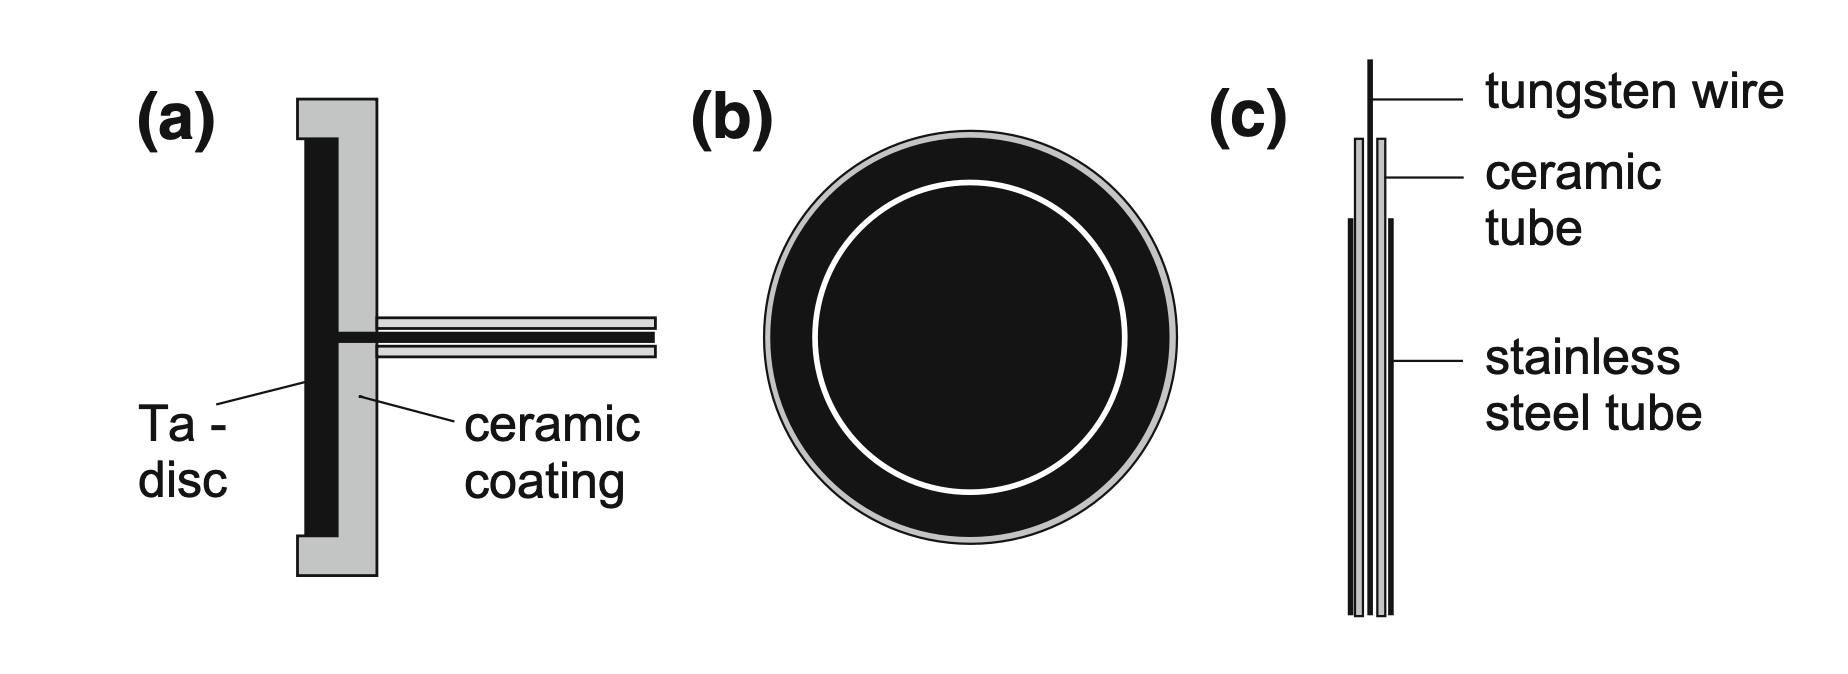
\includegraphics[width=0.65\textwidth]{../figures/langmuir_probe.png}
        \\
        \small Structure of a common plane Langmuir probe \footfullcite{piel_plasma_2017}
    \end{center}
\end{frame}


\begin{frame}{The $I$--$V$ characteristic curve}
    \begin{columns}
        \column{0.5\textwidth}
        Three regions:
        \begin{enumerate}
            \item[I] High negative bias: no electrons reach the probe. Constant ion saturation current.
            \item[II] Electron retardation regime: part of the electrons reach the probe. Electron current (\footfullcite{piel_plasma_2017} or \footfullcite{bagnato_notice_2019})
            \begin{equation*}
                I_e = \electronsaturationcurrent \frac{e^{q(\probevoltage - \biasvoltage)}}{k_B T_e}
            \end{equation*}
            \item[III] High positive bias: constant electron saturation current $\electronsaturationcurrent$.
            \begin{equation*}
                \electronsaturationcurrent = \frac{1}{4}e n_e v_{e,th} A_{\mathrm{probe}}
            \end{equation*}
        \end{enumerate}
        \column{0.5\textwidth}
        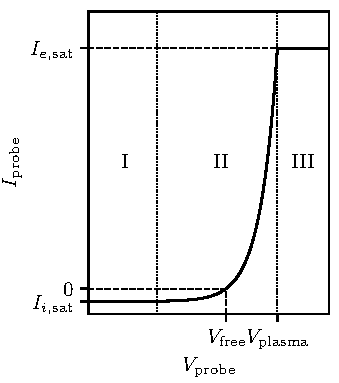
\includegraphics[scale=1]{../figures/langmuir_characteristic.pdf}
    \end{columns}
    % \begin{itemize}
    %     \item Floating potential $\Phi_f$: no current flows in the probe
    %     \item Plasma potential $\Phi_p$: the potential inside the ambient plasma, corresponds to $\electronsaturationcurrent$.
    % \end{itemize}
\end{frame}

\begin{frame}{Extracting electron temperature and density}{[Pas definitif, faut que je choisisse quoi dire]}
    \begin{columns}
        \column{0.5\textwidth}
        Linearise region II by computing logarithm

        Linear regression in region II allows to find $T_e$.
        \begin{equation*}
            \ln\left(\frac{I_e}{I_e,sat} \right) = \frac{e(V_{probe} - V_{bias})}{k_B T_e}
        \end{equation*} 
        Electron saturation current allows to find $n_e$
        \begin{equation*}
            n_e = \frac{4}{e v_e A_p} I_{e,sat} = \frac{1}{e A_p} \sqrt{\frac{2 \pi m_e}{k_B T_e}} I_{e,sat}
        \end{equation*}

        \column{0.5\textwidth}
        
\includegraphics[scale=1]{../figures/IV_fit.pdf}
    \end{columns}
\end{frame}


\begin{frame}{Ion acoustic waves}{CITATION?}
    \begin{itemize}
        \item Longitudal oscillation of charges in plasma
        \item Low pressure $\implies$ almost no collisions, only Coulomb interactions
        \item 1 type of ion: $_{18}$Ar
    \end{itemize}
    
    \vspace{0.5cm}
    \begin{columns}[T]
        \column{0.5\textwidth}
        Dispersion relation
        \begin{equation*}
            v_s^2 = \frac{\gamma_e Z_i k_B T_e + \gamma_i k_B T_i}{M(1+\gamma_e(k\lambda_d)^2)}
        \end{equation*}
        
        \column{0.5\textwidth}
        \vfill
        \centering
        $M$ mass of ion \\
        $Z$ charge of ion \\
        $T_e$/$T_i$ temperature of \electron/ion \\
        $\gamma_e=3$, $\gamma_i=1$
        \vfill
    \end{columns}

    \vspace{0.8cm}
    Under long wavelength and cold plasma assumption
    \begin{equation*}
        \begin{rcases}
            \lambda \gg \lambda_d \\
            T_i \ll 1
        \end{rcases}
        \implies v_s^2 = \frac{\gamma_e Z k_B T_e}{M}
    \end{equation*}
\end{frame}


\begin{frame}{Experimental setup}
    % Prendre figure dans vieux rapport et citer?
    \centering
    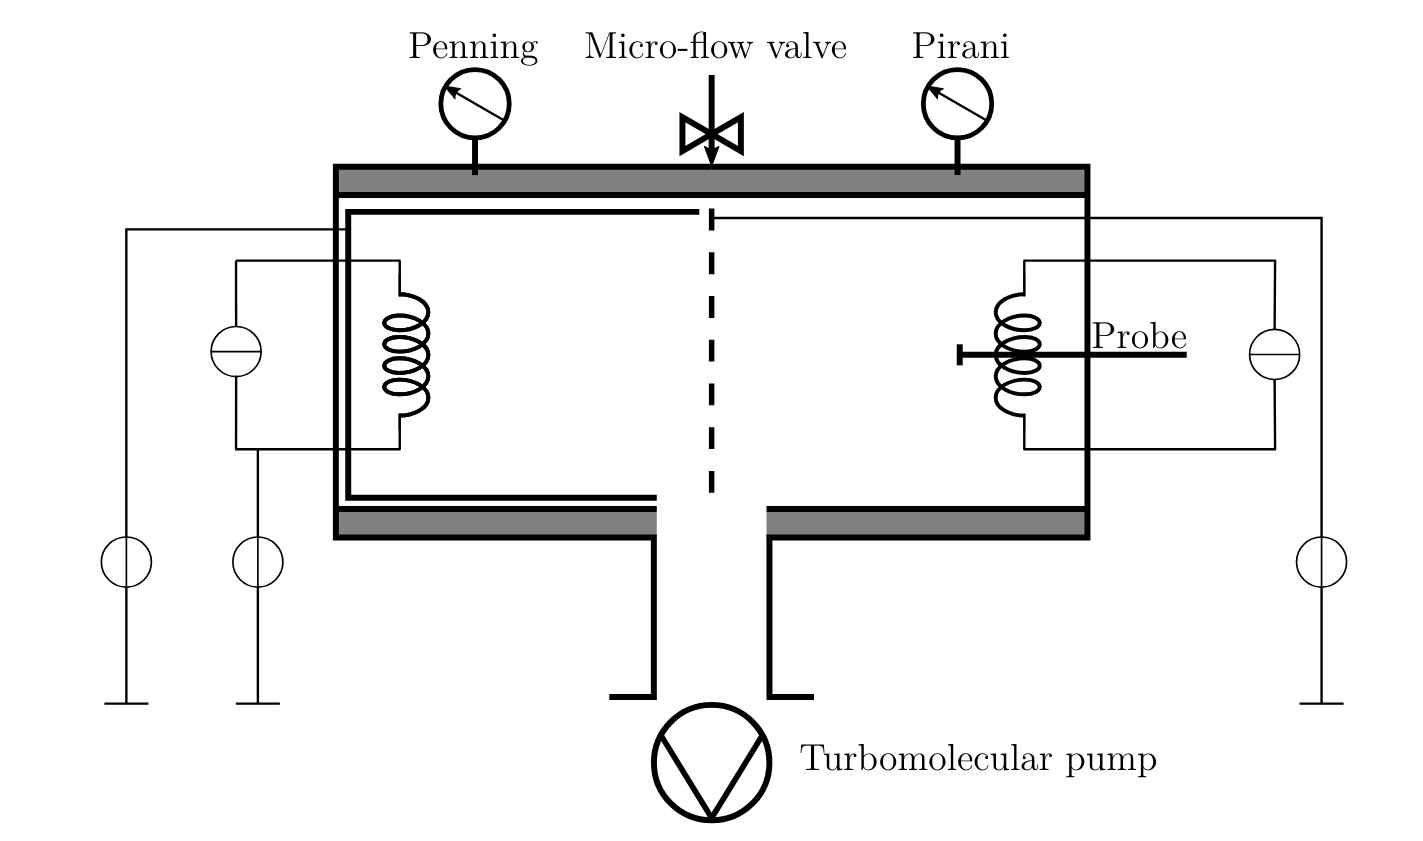
\includegraphics[width=\textwidth]{../figures/experimental_setup_Willemin_Zahar.png} 
    \\
    Diagram/schematics whatever of what we did\footfullcite{experimental_setup_Willemin_Zahar}
    % il est morlement impossible qua u fond ce brave monsieur ai tort
\end{frame}

\section{Results}
\begin{frame}{(Variation avec position, differentes pressions)}{$\filamentcurrent = 50$ A, $\filamentpolarisation = 60$ V, $\gridpolarisation = -100$ V}
    \begin{columns}[T]
        \column{0.5\textwidth}
        \centering
        {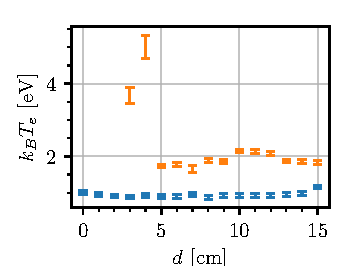
\includegraphics[scale=1]{../figures/temperatureeV_position.pdf}}
        \begin{itemize}
            \item Close to heating element and grid \(\rightarrow\) higher \electron temperature
            \item Higher pressure decreases temperature and increases density
            \item Maximal density for distances $\sim 10$ cm from heating element
        \end{itemize}

        \column{0.5\textwidth}
        \centering
        {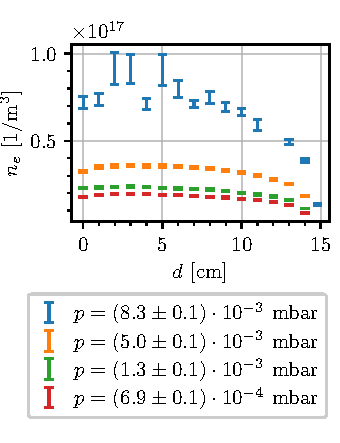
\includegraphics[scale=1]{../figures/density_position.pdf}}
    \end{columns}

\end{frame}
    
\begin{frame}{Effects of pressure}{IMPORTANT! donner les autres parametres (ceux qui n'ont pas été variés pour faire le plot)}

    \begin{columns}
        \column{0.5\textwidth}
        \centering
        {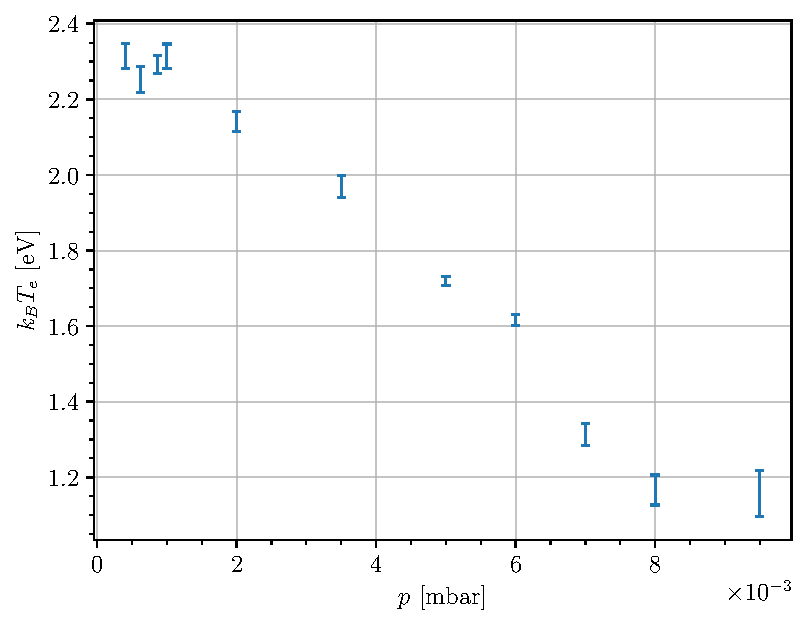
\includegraphics[scale=1]{../figures/temperatureeV_pressure.pdf}}


        \column{0.5\textwidth}
        \centering
        {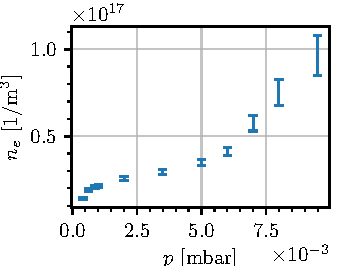
\includegraphics[scale=1]{../figures/density_pressure.pdf}}

    \end{columns}
    \begin{itemize}
        \item Higher pressure decreases temperature and decreases temperature.
        \item Non linear
    \end{itemize}
\end{frame}

\begin{frame}{Heating something}{IMPORTANT! donner les autres parametres (ceux qui n'ont pas été variés pour faire le plot)}
    \begin{columns}
        \column{0.5\textwidth}
        \centering
        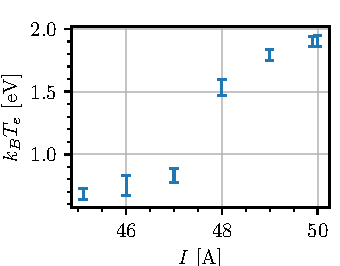
\includegraphics[scale=1]{../figures/temperatureeV_current.pdf}


        \column{0.5\textwidth}
        \centering
        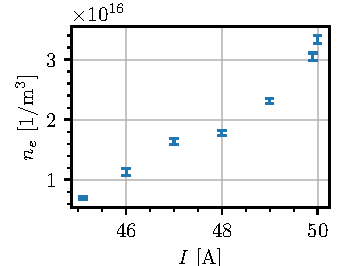
\includegraphics[scale=1]{../figures/density_current.pdf}

    \end{columns}
    \vspace{0.5cm}
    Heating more leads to higher temperature and higher density

    [On ne pouvait pas monter plus en haut]
\end{frame}

\begin{frame}{Variation avec filament polarisation}{IMPORTANT! donner les autres parametres (ceux qui n'ont pas été variés pour faire le plot)}
    \begin{columns}
        \column{0.5\textwidth}
        \centering
        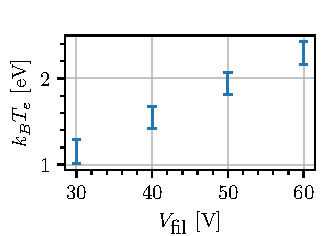
\includegraphics[scale=1]{../figures/temperatureeV_filament_polarisation.pdf}


        \column{0.5\textwidth}
        \centering
        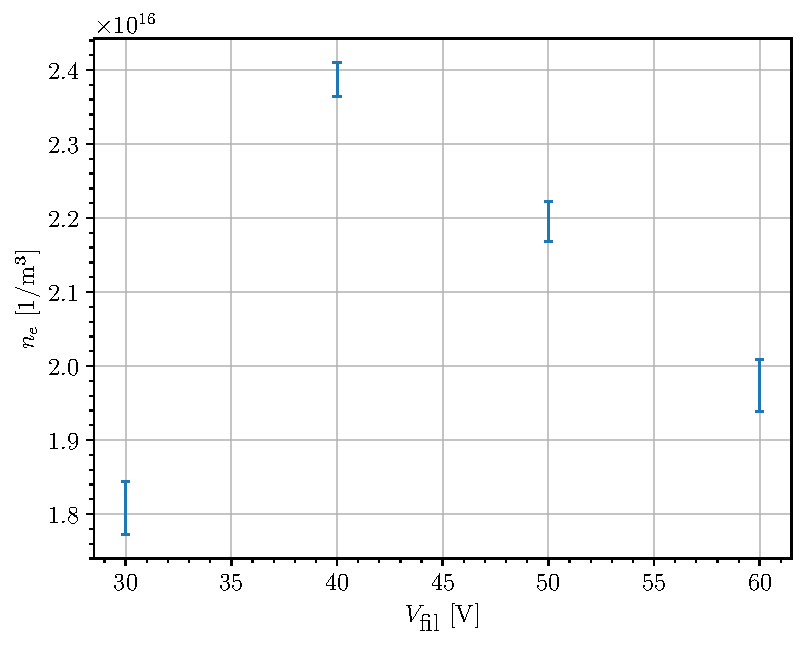
\includegraphics[scale=1]{../figures/density_filament_polarisation.pdf}

    \end{columns}
    \vspace{0.5cm}
    \begin{itemize}
        \item Temperature increases with polarisation
        \item What is happening for density?
    \end{itemize}
\end{frame}

\begin{frame}{Radial Langmuir probe profile boh}
    \begin{columns}
        \column{0.5\textwidth}
        \centering
        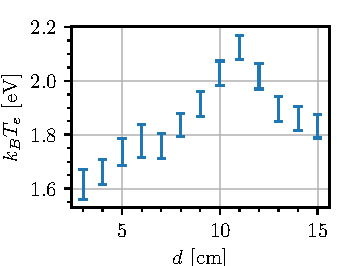
\includegraphics[scale=1]{../figures/temperatureeV_position_radial.pdf}

        \column{0.5\textwidth}
        \centering
        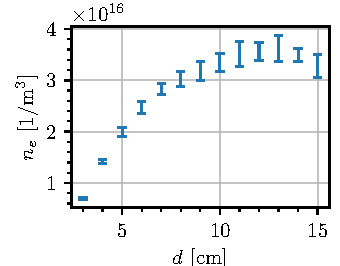
\includegraphics[scale=1]{../figures/density_position_radial.pdf}

    \end{columns}
    \vspace{0.5cm}
    Temperature and density falls off near the external walls.
\end{frame}

\begin{frame}{Difference between using one and two filaments}
    {A study in position}
    \begin{columns}
        \column{0.5\textwidth}
        \centering
        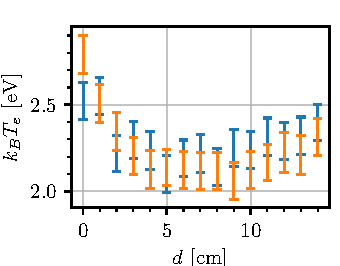
\includegraphics[scale=1]{../figures/temperatureeV_position_twofilaments.pdf}

        \column{0.5\textwidth}
        \centering
        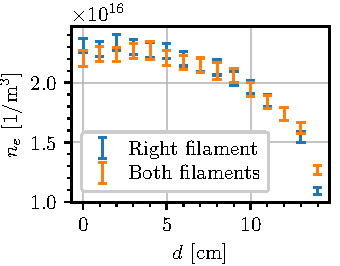
\includegraphics[scale=1]{../figures/density_position_twofilaments.pdf}

    \end{columns}
    \vspace{0.5cm}
    No great difference between using only one or both filaments.
    Maybe maybe maybe on higher $d$.
\end{frame}


\begin{frame}{Temperature and density profile}
    \begin{columns}
        \column{0.5\textwidth}
        \centering
        {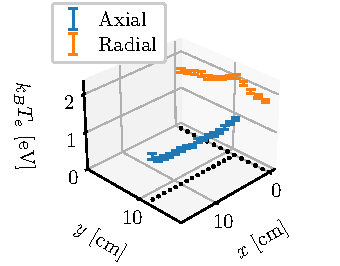
\includegraphics[scale=1]{../figures/temperatureEV_profile.pdf}}

        \column{0.5\textwidth}
        \centering
        {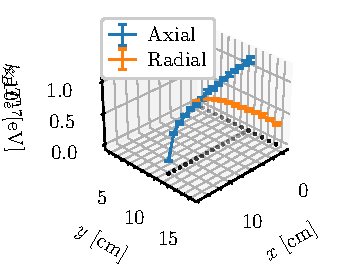
\includegraphics[scale=1]{../figures/density_profile.pdf}}

    \end{columns}
    Say where the maximums and minimums are.

    Difference de geometrie -> orientation langmuir probe. Cherche champ magnetique.
    test

\end{frame}


\section{Discussion}
\begin{frame}{Discussiooooon}
    Found similar results in literature: 
    \begin{itemize}
        \item \footfullcite{hassouba_analysis_2013} describes the same behaviour of temperature and density as a function of pressure.
    \end{itemize}
\end{frame}


\begin{frame}{Observations to put in discussion slides}
    \begin{itemize}
        \item Difficult to propagate ion-acoustic waves in cold plasma [SEARCH AND EXPLAIN WHY].
        \item The grid doesn't have a visible effect on the observed waves.
        \item Why so sensitive
    \end{itemize}
\end{frame}


\begin{frame}{Hysteresis}{WE CAN PUT COOL FIGURE FROM PAPER}
    \begin{itemize}
        \item Hysteresis observed for high filament current and high Ar pressure
        \item Caused by contamination layer on the probe surface \footfullcite{oyama_systematic_1976}
    \end{itemize}
    \begin{center}
        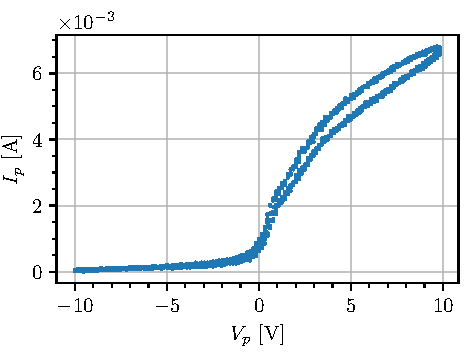
\includegraphics[scale=1]{../figures/hysteresis.pdf}
    \end{center}

\end{frame}


\end{document}